
%% bare_conf.tex
%% V1.3
%% 2007/01/11
%% by Michael Shell
%% See:
%% http://www.michaelshell.org/
%% for current contact information.
%%
%% This is a skeleton file demonstrating the use of IEEEtran.cls
%% (requires IEEEtran.cls version 1.7 or later) with an IEEE conference paper.
%%
%% Support sites:
%% http://www.michaelshell.org/tex/ieeetran/
%% http://www.ctan.org/tex-archive/macros/latex/contrib/IEEEtran/
%% and
%% http://www.ieee.org/

%%*************************************************************************
%% Legal Notice:
%% This code is offered as-is without any warranty either expressed or
%% implied; without even the implied warranty of MERCHANTABILITY or
%% FITNESS FOR A PARTICULAR PURPOSE! 
%% User assumes all risk.
%% In no event shall IEEE or any contributor to this code be liable for
%% any damages or losses, including, but not limited to, incidental,
%% consequential, or any other damages, resulting from the use or misuse
%% of any information contained here.
%%
%% All comments are the opinions of their respective authors and are not
%% necessarily endorsed by the IEEE.
%%
%% This work is distributed under the LaTeX Project Public License (LPPL)
%% ( http://www.latex-project.org/ ) version 1.3, and may be freely used,
%% distributed and modified. A copy of the LPPL, version 1.3, is included
%% in the base LaTeX documentation of all distributions of LaTeX released
%% 2003/12/01 or later.
%% Retain all contribution notices and credits.
%% ** Modified files should be clearly indicated as such, including  **
%% ** renaming them and changing author support contact information. **
%%
%% File list of work: IEEEtran.cls, IEEEtran_HOWTO.pdf, bare_adv.tex,
%%                    bare_conf.tex, bare_jrnl.tex, bare_jrnl_compsoc.tex
%%*************************************************************************

% *** Authors should verify (and, if needed, correct) their LaTeX system  ***
% *** with the testflow diagnostic prior to trusting their LaTeX platform ***
% *** with production work. IEEE's font choices can trigger bugs that do  ***
% *** not appear when using other class files.                            ***
% The testflow support page is at:
% http://www.michaelshell.org/tex/testflow/



% Note that the a4paper option is mainly intended so that authors in
% countries using A4 can easily print to A4 and see how their papers will
% look in print - the typesetting of the document will not typically be
% affected with changes in paper size (but the bottom and side margins will).
% Use the testflow package mentioned above to verify correct handling of
% both paper sizes by the user's LaTeX system.
%
% Also note that the "draftcls" or "draftclsnofoot", not "draft", option
% should be used if it is desired that the figures are to be displayed in
% draft mode.
%
\documentclass[conference]{IEEEtran}
% Add the compsoc option for Computer Society conferences.
%
% If IEEEtran.cls has not been installed into the LaTeX system files,
% manually specify the path to it like:
% \documentclass[conference]{../sty/IEEEtran}





% Some very useful LaTeX packages include:
% (uncomment the ones you want to load)


% *** MISC UTILITY PACKAGES ***
%
%\usepackage{ifpdf}
% Heiko Oberdiek's ifpdf.sty is very useful if you need conditional
% compilation based on whether the output is pdf or dvi.
% usage:
% \ifpdf
%   % pdf code
% \else
%   % dvi code
% \fi
% The latest version of ifpdf.sty can be obtained from:
% http://www.ctan.org/tex-archive/macros/latex/contrib/oberdiek/
% Also, note that IEEEtran.cls V1.7 and later provides a builtin
% \ifCLASSINFOpdf conditional that works the same way.
% When switching from latex to pdflatex and vice-versa, the compiler may
% have to be run twice to clear warning/error messages.






% *** CITATION PACKAGES ***
%
%\usepackage{cite}
% cite.sty was written by Donald Arseneau
% V1.6 and later of IEEEtran pre-defines the format of the cite.sty package
% \cite{} output to follow that of IEEE. Loading the cite package will
% result in citation numbers being automatically sorted and properly
% "compressed/ranged". e.g., [1], [9], [2], [7], [5], [6] without using
% cite.sty will become [1], [2], [5]--[7], [9] using cite.sty. cite.sty's
% \cite will automatically add leading space, if needed. Use cite.sty's
% noadjust option (cite.sty V3.8 and later) if you want to turn this off.
% cite.sty is already installed on most LaTeX systems. Be sure and use
% version 4.0 (2003-05-27) and later if using hyperref.sty. cite.sty does
% not currently provide for hyperlinked citations.
% The latest version can be obtained at:
% http://www.ctan.org/tex-archive/macros/latex/contrib/cite/
% The documentation is contained in the cite.sty file itself.



% *** GRAPHICS RELATED PACKAGES ***
%
\ifCLASSINFOpdf
   \usepackage[pdftex]{graphicx}
  % declare the path(s) where your graphic files are
  % \graphicspath{{../pdf/}{../jpeg/}}
  % and their extensions so you won't have to specify these with
  % every instance of \includegraphics
  % \DeclareGraphicsExtensions{.pdf,.jpeg,.png}
\else
  % or other class option (dvipsone, dvipdf, if not using dvips). graphicx
  % will default to the driver specified in the system graphics.cfg if no
  % driver is specified.
  % \usepackage[dvips]{graphicx}
  % declare the path(s) where your graphic files are
  % \graphicspath{{../eps/}}
  % and their extensions so you won't have to specify these with
  % every instance of \includegraphics
  % \DeclareGraphicsExtensions{.eps}
\fi
% graphicx was written by David Carlisle and Sebastian Rahtz. It is
% required if you want graphics, photos, etc. graphicx.sty is already
% installed on most LaTeX systems. The latest version and documentation can
% be obtained at: 
% http://www.ctan.org/tex-archive/macros/latex/required/graphics/
% Another good source of documentation is "Using Imported Graphics in
% LaTeX2e" by Keith Reckdahl which can be found as epslatex.ps or
% epslatex.pdf at: http://www.ctan.org/tex-archive/info/
%
% latex, and pdflatex in dvi mode, support graphics in encapsulated
% postscript (.eps) format. pdflatex in pdf mode supports graphics
% in .pdf, .jpeg, .png and .mps (metapost) formats. Users should ensure
% that all non-photo figures use a vector format (.eps, .pdf, .mps) and
% not a bitmapped formats (.jpeg, .png). IEEE frowns on bitmapped formats
% which can result in "jaggedy"/blurry rendering of lines and letters as
% well as large increases in file sizes.
%
% You can find documentation about the pdfTeX application at:
% http://www.tug.org/applications/pdftex





% *** MATH PACKAGES ***
%
%\usepackage[cmex10]{amsmath}
% A popular package from the American Mathematical Society that provides
% many useful and powerful commands for dealing with mathematics. If using
% it, be sure to load this package with the cmex10 option to ensure that
% only type 1 fonts will utilized at all point sizes. Without this option,
% it is possible that some math symbols, particularly those within
% footnotes, will be rendered in bitmap form which will result in a
% document that can not be IEEE Xplore compliant!
%
% Also, note that the amsmath package sets \interdisplaylinepenalty to 10000
% thus preventing page breaks from occurring within multiline equations. Use:
%\interdisplaylinepenalty=2500
% after loading amsmath to restore such page breaks as IEEEtran.cls normally
% does. amsmath.sty is already installed on most LaTeX systems. The latest
% version and documentation can be obtained at:
% http://www.ctan.org/tex-archive/macros/latex/required/amslatex/math/





% *** SPECIALIZED LIST PACKAGES ***
%
%\usepackage{algorithmic}
% algorithmic.sty was written by Peter Williams and Rogerio Brito.
% This package provides an algorithmic environment fo describing algorithms.
% You can use the algorithmic environment in-text or within a figure
% environment to provide for a floating algorithm. Do NOT use the algorithm
% floating environment provided by algorithm.sty (by the same authors) or
% algorithm2e.sty (by Christophe Fiorio) as IEEE does not use dedicated
% algorithm float types and packages that provide these will not provide
% correct IEEE style captions. The latest version and documentation of
% algorithmic.sty can be obtained at:
% http://www.ctan.org/tex-archive/macros/latex/contrib/algorithms/
% There is also a support site at:
% http://algorithms.berlios.de/index.html
% Also of interest may be the (relatively newer and more customizable)
% algorithmicx.sty package by Szasz Janos:
% http://www.ctan.org/tex-archive/macros/latex/contrib/algorithmicx/




% *** ALIGNMENT PACKAGES ***
%
%\usepackage{array}
% Frank Mittelbach's and David Carlisle's array.sty patches and improves
% the standard LaTeX2e array and tabular environments to provide better
% appearance and additional user controls. As the default LaTeX2e table
% generation code is lacking to the point of almost being broken with
% respect to the quality of the end results, all users are strongly
% advised to use an enhanced (at the very least that provided by array.sty)
% set of table tools. array.sty is already installed on most systems. The
% latest version and documentation can be obtained at:
% http://www.ctan.org/tex-archive/macros/latex/required/tools/


%\usepackage{mdwmath}
%\usepackage{mdwtab}
% Also highly recommended is Mark Wooding's extremely powerful MDW tools,
% especially mdwmath.sty and mdwtab.sty which are used to format equations
% and tables, respectively. The MDWtools set is already installed on most
% LaTeX systems. The lastest version and documentation is available at:
% http://www.ctan.org/tex-archive/macros/latex/contrib/mdwtools/


% IEEEtran contains the IEEEeqnarray family of commands that can be used to
% generate multiline equations as well as matrices, tables, etc., of high
% quality.


%\usepackage{eqparbox}
% Also of notable interest is Scott Pakin's eqparbox package for creating
% (automatically sized) equal width boxes - aka "natural width parboxes".
% Available at:
% http://www.ctan.org/tex-archive/macros/latex/contrib/eqparbox/





% *** SUBFIGURE PACKAGES ***
%\usepackage[tight,footnotesize]{subfigure}
% subfigure.sty was written by Steven Douglas Cochran. This package makes it
% easy to put subfigures in your figures. e.g., "Figure 1a and 1b". For IEEE
% work, it is a good idea to load it with the tight package option to reduce
% the amount of white space around the subfigures. subfigure.sty is already
% installed on most LaTeX systems. The latest version and documentation can
% be obtained at:
% http://www.ctan.org/tex-archive/obsolete/macros/latex/contrib/subfigure/
% subfigure.sty has been superceeded by subfig.sty.



%\usepackage[caption=false]{caption}
%\usepackage[font=footnotesize]{subfig}
% subfig.sty, also written by Steven Douglas Cochran, is the modern
% replacement for subfigure.sty. However, subfig.sty requires and
% automatically loads Axel Sommerfeldt's caption.sty which will override
% IEEEtran.cls handling of captions and this will result in nonIEEE style
% figure/table captions. To prevent this problem, be sure and preload
% caption.sty with its "caption=false" package option. This is will preserve
% IEEEtran.cls handing of captions. Version 1.3 (2005/06/28) and later 
% (recommended due to many improvements over 1.2) of subfig.sty supports
% the caption=false option directly:
%\usepackage[caption=false,font=footnotesize]{subfig}
%
% The latest version and documentation can be obtained at:
% http://www.ctan.org/tex-archive/macros/latex/contrib/subfig/
% The latest version and documentation of caption.sty can be obtained at:
% http://www.ctan.org/tex-archive/macros/latex/contrib/caption/




% *** FLOAT PACKAGES ***
%
%\usepackage{fixltx2e}
% fixltx2e, the successor to the earlier fix2col.sty, was written by
% Frank Mittelbach and David Carlisle. This package corrects a few problems
% in the LaTeX2e kernel, the most notable of which is that in current
% LaTeX2e releases, the ordering of single and double column floats is not
% guaranteed to be preserved. Thus, an unpatched LaTeX2e can allow a
% single column figure to be placed prior to an earlier double column
% figure. The latest version and documentation can be found at:
% http://www.ctan.org/tex-archive/macros/latex/base/



%\usepackage{stfloats}
% stfloats.sty was written by Sigitas Tolusis. This package gives LaTeX2e
% the ability to do double column floats at the bottom of the page as well
% as the top. (e.g., "\begin{figure*}[!b]" is not normally possible in
% LaTeX2e). It also provides a command:
%\fnbelowfloat
% to enable the placement of footnotes below bottom floats (the standard
% LaTeX2e kernel puts them above bottom floats). This is an invasive package
% which rewrites many portions of the LaTeX2e float routines. It may not work
% with other packages that modify the LaTeX2e float routines. The latest
% version and documentation can be obtained at:
% http://www.ctan.org/tex-archive/macros/latex/contrib/sttools/
% Documentation is contained in the stfloats.sty comments as well as in the
% presfull.pdf file. Do not use the stfloats baselinefloat ability as IEEE
% does not allow \baselineskip to stretch. Authors submitting work to the
% IEEE should note that IEEE rarely uses double column equations and
% that authors should try to avoid such use. Do not be tempted to use the
% cuted.sty or midfloat.sty packages (also by Sigitas Tolusis) as IEEE does
% not format its papers in such ways.





% *** PDF, URL AND HYPERLINK PACKAGES ***
%
\usepackage{url}
% url.sty was written by Donald Arseneau. It provides better support for
% handling and breaking URLs. url.sty is already installed on most LaTeX
% systems. The latest version can be obtained at:
% http://www.ctan.org/tex-archive/macros/latex/contrib/misc/
% Read the url.sty source comments for usage information. Basically,
% \url{my_url_here}.



\usepackage{todonotes}



% *** Do not adjust lengths that control margins, column widths, etc. ***
% *** Do not use packages that alter fonts (such as pslatex).         ***
% There should be no need to do such things with IEEEtran.cls V1.6 and later.
% (Unless specifically asked to do so by the journal or conference you plan
% to submit to, of course. )


% correct bad hyphenation here
\hyphenation{op-tical net-works semi-conduc-tor}


\begin{document}
%
% paper title
% can use linebreaks \\ within to get better formatting as desired
\title{EmotiBot: an Architecture for a Robotic Actor}


% author names and affiliations
% use a multiple column layout for up to three different
% affiliations
\author{
\IEEEauthorblockN{
Andres De La Pe\~na and Enrique Gonzalez
}
\IEEEauthorblockA{
Departamento de Ingeniería de Sistemas,\\Pontificia Universidad Javeriana,\\
Bogot\'a, Colombia\\
Email \{andres.dlps, egonzal\}@javeriana.edu.co
}
\and
\IEEEauthorblockN{Juli\'an M. Angel F. %
and Andrea Bonarini}
\IEEEauthorblockA{Dipartimento di Elettronica, Informazione e Bioingegneria,\\ Politecnico di Milano,\\
Piazza Leonardo da Vinci 32, 20133 Milano, Italy\\
Email: \{julianmauricio.angel, andrea.bonarini\}@polimi.it}
}

% conference papers do not typically use \thanks and this command
% is locked out in conference mode. If really needed, such as for
% the acknowledgment of grants, issue a \IEEEoverridecommandlockouts
% after \documentclass

% for over three affiliations, or if they all won't fit within the width
% of the page, use this alternative format:
% 
%\author{\IEEEauthorblockN{Michael Shell\IEEEauthorrefmark{1},
%Homer Simpson\IEEEauthorrefmark{2},
%James Kirk\IEEEauthorrefmark{3}, 
%Montgomery Scott\IEEEauthorrefmark{3} and
%Eldon Tyrell\IEEEauthorrefmark{4}}
%\IEEEauthorblockA{\IEEEauthorrefmark{1}School of Electrical and Computer Engineering\\
%Georgia Institute of Technology,
%Atlanta, Georgia 30332--0250\\ Email: see http://www.michaelshell.org/contact.html}
%\IEEEauthorblockA{\IEEEauthorrefmark{2}Twentieth Century Fox, Springfield, USA\\
%Email: homer@thesimpsons.com}
%\IEEEauthorblockA{\IEEEauthorrefmark{3}Starfleet Academy, San Francisco, California 96678-2391\\
%Telephone: (800) 555--1212, Fax: (888) 555--1212}
%\IEEEauthorblockA{\IEEEauthorrefmark{4}Tyrell Inc., 123 Replicant Street, Los Angeles, California 90210--4321}}




% use for special paper notices
%\IEEEspecialpapernotice{(Invited Paper)}




% make the title area
\maketitle


\begin{abstract}
Interaction happens all the time and everywhere.  It is an intrinsic part of our life (e.g. school, office and house). However, interaction is based in appraisals that people have to do in base of the current situation and others' emotion. In base of these appraisals they have to select the best way to interact with other, which is a difficult task. Thus not all the people are able to face interaction successfully, due to the appraisal is subjective to each person. As a consequence try to build a robot that could be outstanding interacting with humans could be a difficult task. Thus it is necessary to find an environment that allows focus on some aspects of interaction but at the same time that allow the increment of the complexity in the interaction. For this purpose theatre has been selected to be the test bed for the architecture presented in this paper.  The architectures has been created in base of the belief, desire and intention model, and some of the modules have been simplified thanks to constrains given by the theatre but without losing the main objective of interaction with humans.
\end{abstract}
% IEEEtran.cls defaults to using nonbold math in the Abstract.
% This preserves the distinction between vectors and scalars. However,
% if the conference you are submitting to favors bold math in the abstract,
% then you can use LaTeX's standard command \boldmath at the very start
% of the abstract to achieve this. Many IEEE journals/conferences frown onr 
% math in the abstract anyway.

% no keywords




% For peer review papers, you can put extra information on the cover
% page as needed:
% \ifCLASSOPTIONpeerreview
% \begin{center} \bfseries EDICS Category: 3-BBND \end{center}
% \fi
%
% For peerreview papers, this IEEEtran command inserts a page break and
% creates the second title. It will be ignored for other modes.
\IEEEpeerreviewmaketitle

\section{Introduction}
Human-human interaction is done through the correct use of language (e.g. use of the same semantic and grammar) and the coordination of events between the parts. Facing the coordination between humans and robots in a real environment could be difficult or even impossible.\\
Theatre has been suggested as a suitable environment to test timing and expressiveness in robotics~\cite{Breazeal2003,Fan2013,Hoffman2009,lu2011position,Pinhanez97}. However, few works have been presented using theatre as environment to build and test sociability in robots. Some have used theatre to study timing in human-human interaction~\cite{Knight2011,Knight2011b}, others have focused on humanoid platforms that could be used as actors~\cite{Fan2009,Fan2013}, but none of them have worked on how to use theatre to improve emotion expression in totally autonomous robots.\\
Using theatre as test environment, this work faces two principal problems: first, the emotional expressiveness of a robot-actor. And second, the coordination between different agents (i.e. humans or robots). These potentialities are faced from the popular deliberative process in agent's theory called BDI(Belief, Desires and Intentions) which is in turn inspired by a respected theory of rational actions in humans\\
This papers is organized as follows. In section~\ref{sec:relatedwork} is reviewed the use of robots in theatre and section~\ref{sec:theatre} gives the highlights to be selected theatre as a test bed. Section~\ref{sec:architecture} describes the generalities of the architecture, and sections\ref{sec:description},~\ref{sec:belief},~\ref{sec:action}, and~\ref{sec:motivation} gives a more detail about each sub-system that conforms the architecture. Conclusions and further work are presented in section~\ref{sec:conclusions}. 


\section{Related Work}\label{sec:relatedwork}
Literature about robot actors is not wide. Although there are works that have used robots in theatrical representations, these robots are often used as props. Other works have focused on the development of systems that could interact with the audience \cite{Mavridis2009,Breazeal2003}. The most advanced is the standup comedy implemented by Knight \cite{Knight2011b,Knight2011}. In this, a NAO platform~\cite{NAO2013} sits in front of a whole auditorium. The robot tells a joke and selects autonomously the next joke based on the reaction of the audience. To get this information, the robot relies on cameras, colored paddles and a microphone. The robot performs basic actions to add some expressiveness to the joke, but it does not project any emotion.\\
Other works~\cite{Wurst2002,Bruce2002} have adopted theatre as a place to implement simple actors with all information (even objects' position) hard-coded, and no interaction with people. Although these robots could be perceived as autonomous, they do not make any adjustment during their performance, losing realism, e.g., if the other robot does not play in its precise place. \\
Complex performances have been given in 2011, when \textit{Roboscopie}~\cite{Roboscopie2012,Lemaignan2012} was presented. Roboscopie story involved one person and one robot. The robot could navigate autonomously in its environment and build a 3D model of it. But, the human-robot coordination was done manually during the presentation, and the position of some objects was already known by the robot.\\
Fahn and collaborators worked with humanoid robots as actors~\cite{Fan2009,Fan2013}. They believe humanoid robots are suitable as theatre actors more than other kind of robots. They have developed two humanoid robots, Janet and Thomas~\cite{Fan2009}, and two wheeled robots, Pica and Ringo \cite{Hsu2007}. These robots are capable to perform autonomously many actions such as: draw people, jazz drumming, marionette operating, and notation reading and singing. However, their humanoid robots have problems with the amount of computers needed to control them. The high complexity to control the humanoid platforms and the lack of expression in their action, except for their faces, make this approach unsuitable to study emotion generation.\\
Trying to add some theatrical realism to robots, Breazeal and collaborators~\cite{Breazeal2008} designed and implemented a system to control a lamp. The main characteristic of this lamp is that it could be controlled by just one person, which could select the focus point where the lamp must look at. This little thing improved the credibility that the lamp was listening to the person that was speaking to it.\\
With the idea to familiarize people with robots, \textit{Robots actors project} was created~\cite{Zaven2012,Torres2013}, where Wakamaru~\cite{Wakamaru2013} and Geminoid F~\cite{Ishiguro2013} robots were used in the play. Unfortunately, deeper information about this implementation is not available, although from videos is possible to infer that the play has been designed for robots and robots seem remotely driven.
\section{Theatre}\label{sec:theatre}
Theatre is considered as lively art~\cite{wilson2009theatre}. Thanks its characteristics and constraints, it is an excellent framework to test sociability and expressiveness in robots; moreover, actor training systems (e.g.,~\cite{wilson2009theatre,cavanaugh2012acting,genevieve2009delsarte,Stanislavski1989} can inspire the development of expressive robots.
%%%%%%%%%%%%%%%%%%%%%%%%%%%%%%%%%
\subsection{Characteristics}
People are used to think at theatre as a repetitive show, and essential points that make theatre a lively art are often forgotten~\cite{wilson2009theatre}: 
\begin{itemize}
\item On the opposite of television or movies, during a theatre performance actors do not have a second chance to perform in front of the same audience. If an actor fails remembering a line, or he/she does not show a believable character, the audience are going to get a bad impression of the play.
\item Each performance is unique. No matter how much effort actors do to repeat each time the same performance, subtle changes could be seen: actors' and objects' stage position, actors' mood and, more importantly, audience's attitude. 
\item Audience's attitude affects actors. Actor could hear laughs, coughs, silence, and could even feel the tension in the audience. This could eager or discourage actors, affecting the whole performance. 
\item The performance outcome does not rely on one person. Good outcome comes from correct collaboration and coordination of playwriter, director, technical people and performers. In the specific performers case, they must work as a unity and show to the public a coherent story. 
\end{itemize}
Therefore, theatrical robot actors should have abilities similar to those of their human counterpart to be considered as actors and not as props. This makes necessary that robot actors be expressive, social, and with enough autonomy to be able to face anything may happen on stage.
%%%%%%%%%%%%%%%%%%%%%%%%%%%%%%%%%
\subsection{Constraints}
Theatre constraints makes it possible to focus research efforts on emotion expression and social behavior, considering that robots have already at least a general idea of what to do and how. These constraints are: 
\begin{itemize}
	\item The play script contains all the necessary information: actions, coordination cues, dialogues, and characters attitude. 
	\item Since the script is known before any representation, rehearsals can be done to get used with objects' and performers' positions.
	\item The stage space is discretized to facilitate directors to give instructions, and actors to remember their positions (Figure \ref{fig:StageDirections}).
\begin{figure}
	\centering
	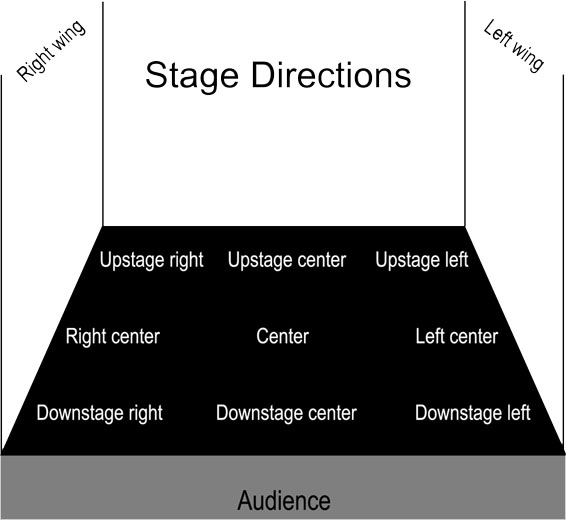
\includegraphics[width=0.4\textwidth]{Images/StageDirection.png} 
	\caption{Stage division used by directors to give instructions~\cite{Musical}.}
	\label{fig:StageDirections}
\end{figure}
	\item Actors should basically take one out of eight preset orientations during a performance (Figure~\ref{fig:BodyPosition}).   
	\begin{figure}
	\centering
	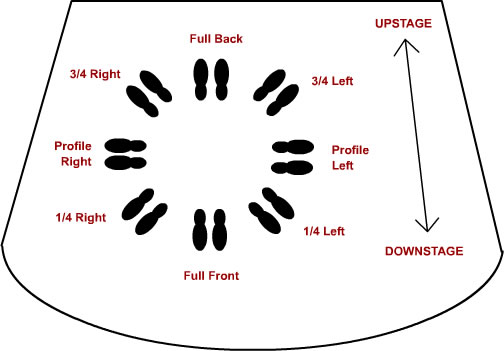
\includegraphics[width=0.4\textwidth]{Images/BodyPosition.png} 
	\caption{Eight possible actors' body position~\cite{Artopia}.}
	\label{fig:BodyPosition}
\end{figure}
\end{itemize}
\section{Architecture}\label{sec:architecture}
This section describes the overall proposal architecture for robo-actors. This description is divided into two views. 

The first view show the structural composition of an roboactor and describes generally which responsibilities its internal structures have(responsibilities of all the blue boxes in the image).

The architecture could be seen in the Figure~\ref{fig:generalArchitecture}. 
\todo[inline]{I made some changes in the image of the architecture}
 \todo[inline]{In the caption of the architecture should be finished the explanation of the arrows, which is not so clear if there is additional meaning}
\begin{figure}
	\centering
	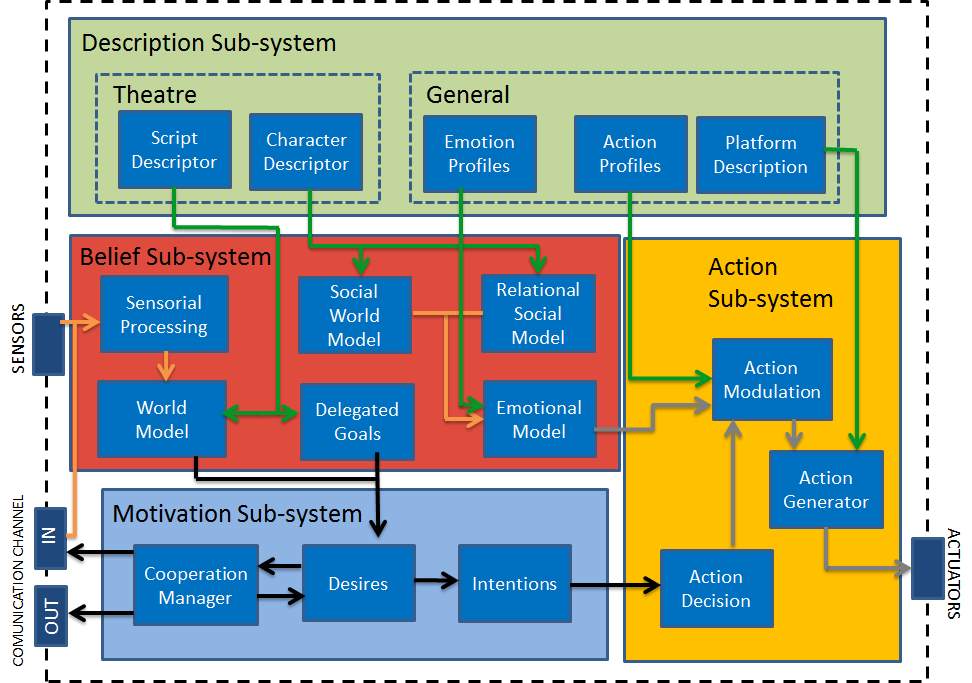
\includegraphics[width=0.5\textwidth]{Images/GeneralArchitecture.png} 
	\caption{General architecture . The green arrows show the information that comes from the description sub-system. The orange arrows are information that is share in the belief sub-system.}
	\label{fig:generalArchitecture}
\end{figure}

The second view is the behavioral structure in a general way. Also, It can be divided in two parts:

First, describes the internal behavior of beliefs in a robo-actor in which is important highlight the emotional and knowledge representation in relationship with the theatre context.

The second part is dedicated to the cooperation mechanisms and deliberation process through which the robots are able to coordinate and act.
\section{Configuration Module}\label{sec:configuration Module}
The action description defines all the necessary information that are required to generate emotive actions and personalize the system. This system is divided into parts: general, which described the information to generate the emotive actions. And Theatre, which describes the script and the current character that should be portrayed by 
the robot.
\subsection{Theatre}
The theatre configuration is the component responsible for store and manage the traditional theatre artefact like the script, the character descriptor, the scenario and even the directors guidelines.
\subsection{General}
The general configuration is components that are not limited just a theatre, and there are divided in three groups:
\begin{itemize}
	\item \textit{Actions}: describe the information about the actions that are available in the system. This information enable the user to create new actions based on the existing ones. 
	\item \textit{Platform}: specify which actions could perform each platform, which allow the use the same script in different platforms.
	\item \textit{Emotions}: have the information in how modify the actions to convey emotions. 
\end{itemize} 

\section{Belief}\label{sec:belief}
General description of the structures used for knowledge representation from the agent's perspective. Also we need to specify the models used that allow this knowledge to change and generate new beliefs about the world and itself.

\subsection{Sensory information and processing}
Sense information depends of the capabilities of the robotic platform, that means what the sensors are and what kind of information captures. Depending these information, process and classify useful information 

\subsection{The world model}
The world model in the robo-actor agent refers to space and object representation present in the scenario. This representation is achieve as space-relational graph between objects. this relations 

Description of social world model(How is represented the others' emotions).

\subsection{The delegated goals}
The delegated goals are those responsibilities that the agent have respect a his character. This delegated goals are managed by the script and specifies what the agent has to reached in a very instant of the play.

The structure of the goal is define as follows:
\begin{itemize}
\item The pre-condition of the goal, which indicate the facts that must be true for consider the goal as a potential goal to become a desire.

\item The post-condition, which is the desire state of the world, it means those facts that the agent want to be true.

\item The plan of action, which is a predefined graph of simple actions that trace the path the agent have to follow in order to reach the goal's post-condition. With the graph representation the actions could be executed in parallel.
\end{itemize}

This structure of the goal also applies to the desires and intention, which are goals in different stages of the deliberative process. 

\todo[inline]{Description of how is represented relationship between characters in the Relational social world model.}
\section{Motivation}\label{sec:motivation}
This section describe the deliberation process in the BDI context.
\todo[inline]{I think that in this section would should to put all the focus, which is the main topic of the workshop}
\todo[inline]{Explain how the script gives information for the cooperation.}
\subsection{Cooperation Manager}
\todo[inline]{Example}
Description of when a goal is considered a desire and how its represented.

Description of how and when a goal becomes an intention.

Detail description of the cooperation process and how this affect the normal deliberation process, specifically the evaluation of agent desires.
\section{Example}
\input{Sections/Example}
%\section{Action}\label{sec:action}
%This section describes the modulation process, it means the action definition involving the emotional state of the agent. \todo[inline]{it is missing the explanation of the action module}
\todo[inline]{I don't think that it is important to describe how works each module of this sub-system. I think that it is enough just to explain the general idea.}
Describe the process of action descomposition(Action Decision) in which the simple actions are defined and executed(possibly in parallel).

Describe the modulation component, how the emotional and relational model modifies the parameters of simple actions.

Finally, describe the action generation component.
\section{Conclusions and Further Works}\label{sec:conclusions}
Conclusion and future work for emotibot.
\bibliographystyle{IEEEtran}
\bibliography{Bibliography/Biblography,Bibliography/Bibliography}

% that's all folks
\end{document}


